% !TEX encoding = UTF-8 Unicode
\documentclass[a4paper,12pt]{article}

%-----------------------------------------Include package & set up some thing-----------------------------------------------
\usepackage{fontspec}
\setmainfont{Times New Roman} %set font
\usepackage{enumitem} % to format list
\usepackage{amsmath}
\usepackage{listings} % quote code
\usepackage{color}
\usepackage{hyperref} % cite hyperlink & bookmarks
\usepackage{setspace} % space
\usepackage{graphicx} % insert image
\usepackage{subcaption} % Multiple images
\usepackage{float}
\usepackage[margin=1in, footskip = 0.25in]{geometry} % Change margin with geometry package

\hypersetup{unicode, colorlinks,linkcolor=black, urlcolor=cyan} % format hyperlink and bookmarks

%Define title
\title{Báo cáo bài tập 9}
\author{1612174 - Phùng Tiến Hào - \href{mailto:tienhaophung@gmail.com}{tienhaophung@gmail.com}}
\date{09/06/2019}

%Code formatting with the listing package
\definecolor{codegreen}{rgb}{0,0.6,0}
\definecolor{codegray}{rgb}{0.3,0.3,0.3}
\definecolor{codepurple}{rgb}{0.58,0,0.82}
\definecolor{backcolour}{rgb}{0.92,0.92,0.88}

\lstdefinestyle{mystyle}{
	backgroundcolor=\color{backcolour},   
	commentstyle=\color{codegreen},
	keywordstyle=\color{blue},
	numberstyle=\tiny\color{codegray},
	stringstyle=\color{codepurple},
	basicstyle=\footnotesize,
	breakatwhitespace=false,         
	breaklines=true,                 
	captionpos=b,                    
	keepspaces=true,                 
	numbers=left,                    
	numbersep=5pt,                  
	showspaces=false,                
	showstringspaces=false,
	showtabs=false,                  
	tabsize=2,
	columns=fullflexible,
	frame=single
}

\lstset{style=mystyle}

\begin{document}
	\pagenumbering{gobble}
	\maketitle
	\newpage
	
	\doublespacing
	\tableofcontents
	\singlespace
	
	\newpage
	\pagenumbering{arabic}
	
	\textbf{Dữ liệu khảo sát:} SpeedDating trong package Lock5withR\\
	
	Load package và thêm các thư viện cần thiết trước khi đi vào xử lý:
	\begin{lstlisting}[language=R]
	require(Lock5withR)
	library(Lock5withR)
	library(mosaic)
	
	# View data
	# View(SpeedDating)
	# Avoid using $
	attach(SpeedDating)
	\end{lstlisting}
	
	\begin{figure}[H]
		\centering
		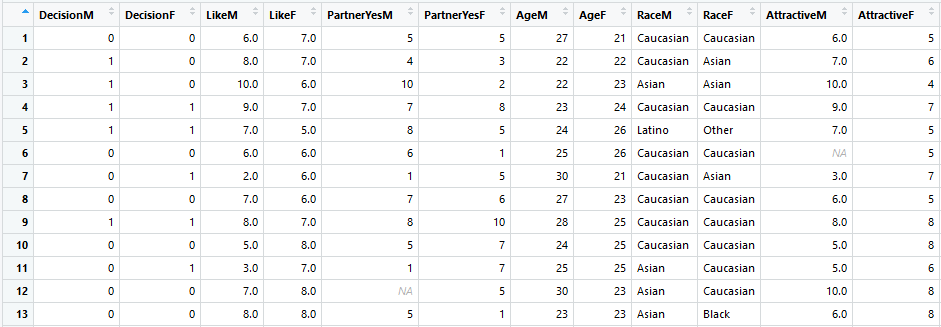
\includegraphics[width=0.7\linewidth]{view_data}
		\caption{View data with the first 13 rows.}
		\label{fig:viewdata}
	\end{figure}
	
	\section{Categorical variables with 2 levels}
	
	\textbf{Biến khảo sát: }LikeM (Num: 1-10), Decision (Yes/No)\\
	Ta có phương trình tuyến tính như sau: $y = b_0 + b_1*x$. Với $b_0$ là hệ số chặn intercept hay còn gọi là bias và $b_1$ là hệ số slope.\\
	
	Trước tiên, ta sẽ plot dữ liệu để khảo sát:
	\begin{lstlisting}[language=R]
		# Plot data
		plot(LikeM~DecisionMale)
		# Plot residual to check if data contains pattern or not  
		plot(model$residuals, pch = 16, col = "blue")
	\end{lstlisting}
	
	\begin{figure}[H]
		\centering
		\begin{subfigure}[b]{0.7\linewidth}
			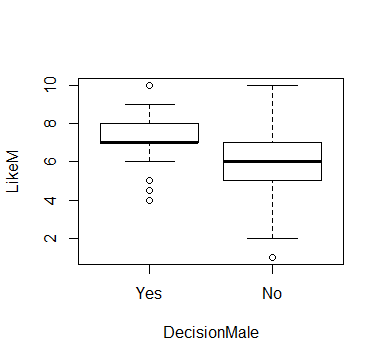
\includegraphics[width=\linewidth]{boxplot.png}
			\caption{Boxplot of LikeM and DecisionMale}
			\label{fig:boxplot}
		\end{subfigure}
		
		\begin{subfigure}[b]{0.7\linewidth}
			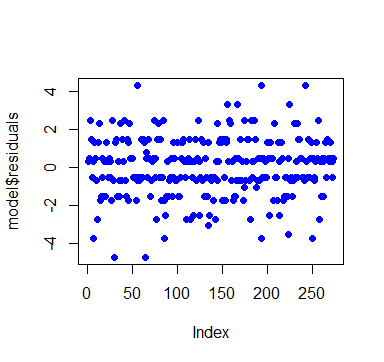
\includegraphics[width=\linewidth]{residual_plot.png}
			\caption{Residual plot}
			\label{fig:resiplot}
		\end{subfigure}
		\caption{Visualize data}
	\end{figure}
	
	Ta nhìn vào hình~\ref{fig:resiplot}, ta thấy dữ liệu được phân bố ngẫu nhiên, không chứa pattern ẩn nào. Do đó, ta có thể yên tâm sử dụng linear regression.\\
	
	Chúng ta cần kiểm tra xem sự khác biệt về LikeM - mức độ thích của nam đối với nữ giữa phản hồi Yes và No.\\ 
	
	Ở đây, ta sẽ tạo ra dummy variables như sau:
	$x = \begin{cases}
		0: \text{No}\\
		1: \text{Yes}
	\end{cases}$
	
	Khi dự đoán LikeM - mức độ thích bằng phương trình hồi qui, ta sẽ có:
	\begin{itemize}
		\item $b_0$ nếu phản hồi No.
		\item $b_0 + b_1$ nếu phản hồi Yes
	\end{itemize}
	
	Có thể giải thích hệ số trên như sau:
	\begin{itemize}
		\item $b_0$ là mức độ thích trung bình của phản hồi No
		\item $b_0 + b_1$ là mức độ thích trung bình của phản hồi Yes
		\item $b_1$ là sự khác biệt về trung bình mức độ thích giữa phản hồi Yes và No.
	\end{itemize}
	
	Kiểm tra sự khác biệt về mức độ thích giữa phản hồi No và Yes bằng việc tính model hồi qui tuyến tính:
	\begin{lstlisting}[language=R]
	# Compute Linear regression model
	model <- lm(LikeM~DecisionMale)
	summary(model)
	\end{lstlisting}
	
	\begin{figure}[H]
		\centering
		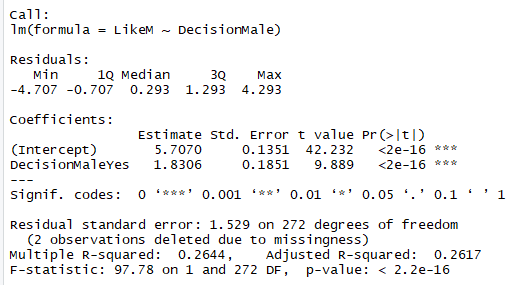
\includegraphics[width=0.7\linewidth]{model1}
		\caption{Summary model}
		\label{fig:model1}
	\end{figure}
	
	Ta thấy rằng DeisionMaleYes có liên kết mạnh với mức độ thích LikeM khi mà $p-value < 2e-16$. Với mức ý nghĩa 0.05, thì ta hoàn toàn tin tưởng rằng có sự khác biệt về mức độ thích giữa phản hồi Yes và No.\\
	
	Cụ thể hơn, ta thấy rằng mức độ thích trung bình của phản hồi No ước tính là $5.7070$ và của phản hồi Yes là $5.7070 + 1.8306 = 7.537671$.\\
	
	Để kiểm tra xem model có tốt không thì ta sẽ nhìn vào hệ số R-squared = 0.2644. Tức là model giải thích được 26.44 độ biến thiên của dữ liệu. Có thể thấy rằng model này vẫn chưa tốt, trong thức tế nếu hệ số R-squared này lớn 0.5 là có thể xem là tốt.\\
	
	Để kiểm tra dummy variables của DecisionMale được phát sinh tự động bởi R:
	\begin{lstlisting}[language=R]
	> # Use contrasts() function to return codes that R have used to create dummy var
	> contrasts(DecisionMale)
	Yes
	No    0
	Yes   1
	\end{lstlisting}
	
	Ta có thể qui định phản hồi Yes là baseline (tức là bằng 0) và No là bằng 1.
	\begin{lstlisting}[language=R]
	# We can specify the baseline to Yes by function relevel()
	SpeedDating2 <- SpeedDating %>% mutate(DecisionMale = relevel(DecisionMale, ref = "Yes"))
	\end{lstlisting}
	
	Tiếp đến, ta sẽ tính lại các hệ số của hồi qui:
	\begin{lstlisting}[language=R]
		model2 <- lm(LikeM~DecisionMale, data = SpeedDating2)
		summary(model2)
	\end{lstlisting}
	
	\begin{figure}[H]
		\centering
		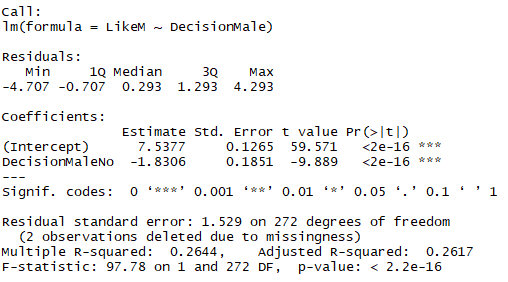
\includegraphics[width=0.7\linewidth]{model}
		\caption{Summary model}
		\label{fig:model}
	\end{figure}
	
	Ở đây, ta thấy hệ số của DecisionMaleNo là $-1.8306 < 0$ do đó nếu là phản hồi No thì mức độ thích sẽ giảm.\\
	
	Khi đó, ước tính cho DecisionMaleYes là $b_0 = 7.5377$ và cho DecisionMaleNo là $b_0 + b_1 = 5.707031$. Ta thấy kết quả ước tính vẫn không thay đổi.
	
	\section{Categorical variables with more than 2 levels}
	
	Ở đây, ta sẽ thực hiện kiểm tra đối với biến định tính có từ 2 levels trở lên. Cụ thể, ta sẽ thực hiện khảo sát mức độ thích LikeM bởi các biến giải thích: AttractiveM - mức độ quyến rũ (Num: 0-10),  DecisionMale - Quyết định làm quen của nam (Yes, No),  RaceF - chủng tộc của nữ (Black, Asian, ...) + SincereM - mức độ chân thành của nữ (Num: 0-10).\\
	
	Trước tiên, việc phải làm là plot dữ liệu
	\begin{lstlisting}[language=R]
	plot(LikeM~AttractiveM + DecisionMale + RaceF + SincereM)
	\end{lstlisting}
	
	\begin{figure}[H]
		\centering
		
			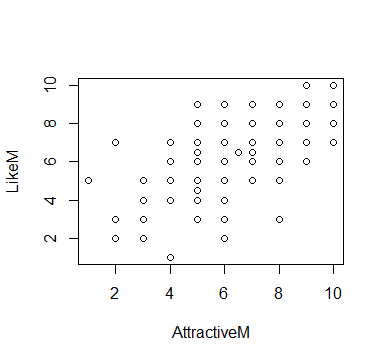
\includegraphics[width=0.7\linewidth]{Rplot1}
			\caption{Scatter plot của LikeM và AttractiveM}
			\label{fig:rplot1}
	\end{figure}
	
	\begin{figure}[H]
		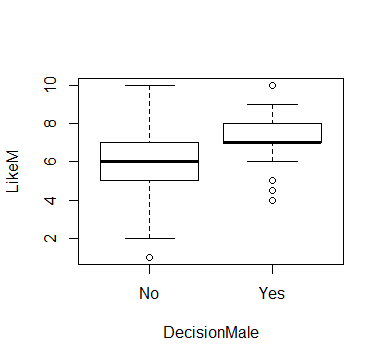
\includegraphics[width=0.7\linewidth]{Rplot2}
		\caption{Boxplot của LikeM và DecisionMale}
		\label{fig:rplot2}
	\end{figure}
	
	\begin{figure}[H]
		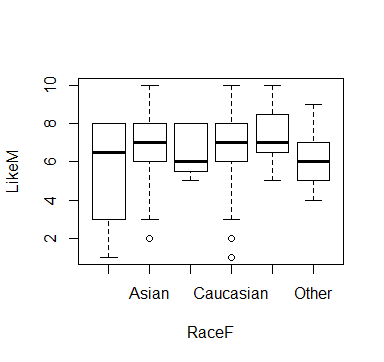
\includegraphics[width=0.7\linewidth]{Rplot3}
		\caption{Boxplot của Like và RaceF}
		\label{fig:rplot3}
	\end{figure}
	
	\begin{figure}[H]
		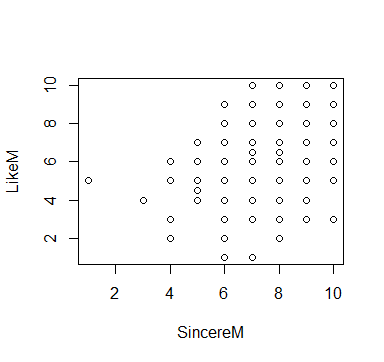
\includegraphics[width=0.7\linewidth]{Rplot4}
		\caption{Scatterplot của LikeM và SincereM}
		\label{fig:rplot4}
	\end{figure}	
	
	Ở đây, nếu một biến định tính có 6 level như RaceF thì ta sẽ tạo dummy code như sau:
	\begin{itemize}
		\item 000000: None (Trường bị bỏ trống trong dữ liệu)
		\item 000001: Asian
		\item 000010: Black
		\item 000100: Caucasian
		\item 001000: Latino
		\item 010000: Other
	\end{itemize}
	
	Để phát sinh các dummy code tự động trong R ta có thể dùng hàm model.matrix():
	\begin{lstlisting}[language=R]
	# Check dummy code of RaceF
	> dummy_code <- model.matrix(~RaceF)
	> head(dummy_code[, -1], 6)
	\end{lstlisting}
	
	\begin{figure}[H]
		\centering
		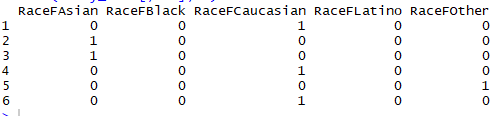
\includegraphics[width=0.7\linewidth]{dummy_coding}
		\caption{Dummy coding của biến RaceF}
		\label{fig:dummycoding}
	\end{figure}
	
	Tiếp đến, ta sẽ đi phân tích phương sai của dữ liệu cũng như kiểm định mối liên kết giữa các biến bằng Anova:
	\begin{lstlisting}[language=R]
	model <- lm(LikeM~AttractiveM + DecisionMale + RaceF + SincereM)
	anova(model)
	\end{lstlisting}
	
	\begin{figure}[H]
		\centering
		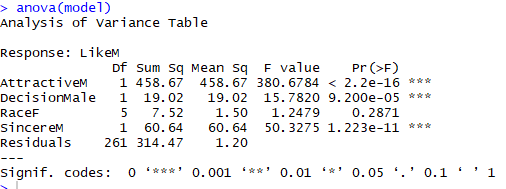
\includegraphics[width=0.7\linewidth]{anova1}
		\caption{Analyst of variance for linear regression model}
		\label{fig:anova1}
	\end{figure}
	
	Ta thấy rằng, RaceF liên kết không đáng kể với sự biến thiên dữ liệu của LikeM khi mà $p-value = 0.2871 > alpha = 0.05$. Nghĩa là ta có $28.71\%$ mà việc dữ đoán của model sẽ không có ý nghĩa. Trong đây, ta chỉ thấy rằng 2 biến DecisionMale, SincereM và AttractiveM có liên kết đáng kể nhất. Cụ thể hơn AttractiveM có $p-value = 2.2e-16$ rất bé cho thấy nó là thành phần cực tốt cần đưa vào model.\\
	
	Ta sẽ xem qua các hệ số của model:
	\begin{lstlisting}[language=R]
	summary(model)
	\end{lstlisting}
	
	\begin{figure}[H]
		\centering
		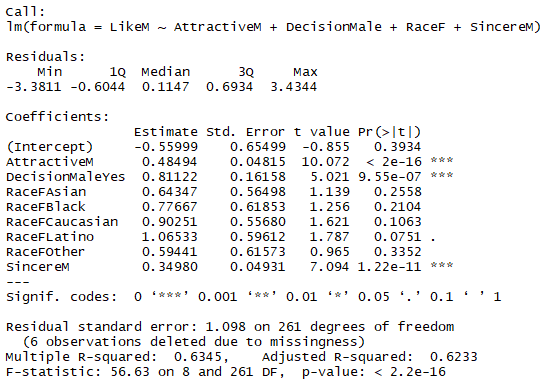
\includegraphics[width=0.7\linewidth]{sum1}
		\caption{Summary of model}
		\label{fig:sum1}
	\end{figure}
	
	Ta thấy rằng: DecisionMaleYes có liên kết dương đáng kể khi mà nó sẽ tăng $0.81122$ mức điểm trung bình của LikeM so với của DecisionMaleNo. Ta thấy rằng biến RaceF có hệ số cũng đáng kể nhưng nó lại chẳng có ý nghĩa cho việc dự đoán của model vì mức độ khó xảy ra của nó khá cao. Đồng nghĩa với việc nó chẳng đóng góp gì đáng kể cho model. Nên ta có thể loại bỏ nó ra khỏi model và kiểm định lại.
	
	\begin{lstlisting}[language=R]
	# Because RaceF is not significantly associated with LikeM, we remove it
	model2 <- lm(LikeM~AttractiveM + DecisionMale + SincereM)
	summary(model2)
	\end{lstlisting}
	
	\begin{figure}[H]
		\centering
		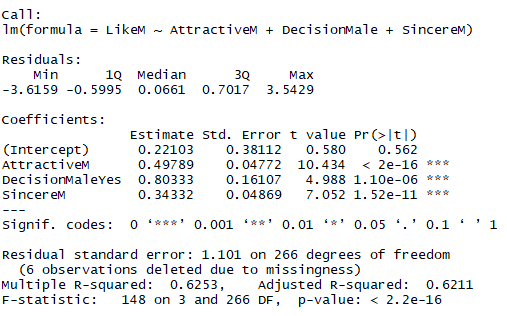
\includegraphics[width=0.7\linewidth]{sum2}
		\caption{Summary of model}
		\label{fig:sum2}
	\end{figure}
	 
	Nhận xét:
	\begin{itemize}
		\item Do dữ liệu có tính phân tán nên residuals của nó khá lớn. Chứng tỏ có sự chênh lệch khá đáng kể giữa giá trị dự đoán và giá trị quan sát.
		\item Thêm nữa, hệ số R-squared = 62.53\%, nghĩa là model chiếm 62.53 độ biến thiên dữ liệu của tổng độ biến thiên của dữ liệu. Tuy rằng, không cao nhưng nếu so thực tế thì lớn 0.5 đã được cân nhắc là khá tốt. 
	\end{itemize}
	
	\begin{thebibliography}{00}
		\bibitem{b1} Randall Pruim and Lana Park. Lock5WithR. Chapter 9: Inference for regression and Chapter 10: Multiple regression. PDF.
		\bibitem{b2} R Users Guide. Chapter 9: Inference for regression and Chapter 10: Multiple regression. PDF.
		\bibitem{b3} Regression with Categorical Variables: Dummy Coding Essentials in R. Retrieved from http://www.sthda.com/english/articles/40-regression-analysis/163-regression-with-categorical-variables-dummy-coding-essentials-in-r/
		\bibitem{b4} "Linear Regression R." DataCamp Community. Retrieved from https://www.datacamp.com/community/
		tutorials/linear-regression-R
	\end{thebibliography}
\end{document}